\documentclass{hnureport}
\usepackage{xeCJK} %调用 xeCJK 宏包
\setCJKmainfont{SimSun} %设置 CJK 主字体为 SimSun (宋体

\renewcommand{\abstractname}{\large Abstract\\}%重定义摘要二字的大小
\begin{document}
\begin{titlepage}
    \clearpage\thispagestyle{empty}
    \centering
    \vspace{1cm}
    % Titles
    {\
        \textsc{Introduction To The Theory Of Computation Michael Sipser}
    }
    \vspace{2.5cm}
    
    \rule{\linewidth}{2mm} \\[0.5cm]
    { \Huge \bfseries Introduction To The Theory Of Computation Michael Sipser\\[0.2em]
        计算理论导论}\\[0.5cm]
    \rule{\linewidth}{0.6mm} \\[1.5cm]
    
    \hspace{2cm}
    \begin{tabular}{l p{5cm}}
        \textbf{LAB} & 实验C----NFA转换为DFA \\[10pt]
        \textbf{Name} & 屈 德 林 \\[10pt]
        \textbf{Student No.} & 201808010522 \\[10pt]
        \textbf{Class} & 计算机科学与技术 1805 \\[10pt]
        \textbf{Department} & CSEE \\[10pt]
        \textbf{Email} & \texttt{qdl.cs@qq.com} \\[10pt]
        \textbf{Date} & \today \\            
    \end{tabular}
    
    % logo
    \vfill
    \centering 
\includegraphics[height=3.5cm]{Figure/HNUlogo.pdf}\\ % light logo
    \centering 
\includegraphics[scale=0.3]{Figure/logo_slogan.png}
    \vspace{0.5cm}

    \pagebreak
\end{titlepage}

% \input{abstract.tex}    %摘要
\thispagestyle{empty}
\tableofcontents
\newpage 
\setcounter{page}{1}
% 问题描述:Target
\section{Problem description}
有限状态自动机(FSM "finite state machine" 或者FSA "finite state automaton" )是为研究有限内存的计算过程和某些语言类而抽象出的一种计算模型。有限状态自动机拥有有限数量的状态,每个状态可以迁移到零个或多个状态,输入字串决定执行哪个状态的迁移。有限状态自动机可以表示为一个有向图。有限状态自动机是自动机理论的研究对象。 
\subsection{定义}
有限状态自动机(FA—finite automaton)是一个五元组:
\begin{itemize}
    \item M=(Q, Σ, δ, q0, F), 其中:
    \item Q——状态的非空有穷集合。
    \item q$\in$Q,q称为M的一个状态。
    \item Σ——输入字母表。
    \item δ——状态转移函数,有时又叫作状态转换函数或者移动函数,δ:Q×Σ→Q,δ(q,a)=p。
    \item q0——M的开始状态,也可叫作初始状态或启动状态。q0 $\in$  Q。
    \item F——M的终止状态集合。F被Q包含。任给q $\in$ F,q称为M的终止状态。
    非确定有限状态自动机(NFA)与确定有限状态自动机(DFA)的唯一区别是它们的转移函数不同。确定有限状态自动机对每一个可能的输入只有一个状态的转移。非确定有限状态自动机对每一个可能的输入可以有多个状态转移,接受到输入时从这多个状态转移中非确定地选择一个。下图是一个非确定性有限状态自动机(NFA)的例子:    
\end{itemize}

\begin{figure}[htbp]	% 浮动
    \centering
    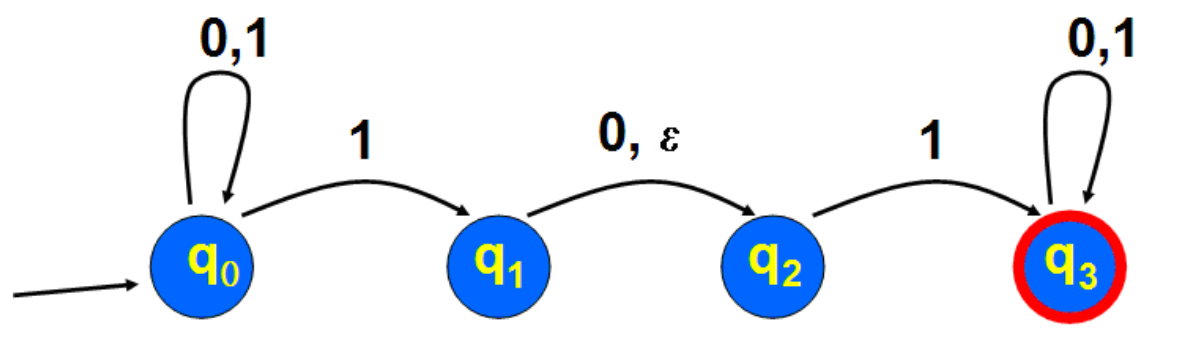
\includegraphics[width=1\linewidth]{Figure/question.png}
    \caption{一个NFA的图文表示}
    \label{fig:figure1latexintro}
\end{figure}
\subsection{状态转移表}
转移函数δ定义自下列状态转移表1。表示状态集合的子集合,采用二进制(特征)串的方式,一个子集中包含该状态,对应的特征串就为1,否则为0,比如上面状态集合的子集{q0q1q2},其特征串就是0111,而子集{q0},其特征串就是0001。将对应的特征串转换为十进制的数字,得到转移函数δ, 如表2:
\begin{figure}[htbp]
	\centering
    \subfigure[表1\#1]{
        \label{fig:sub1}		
		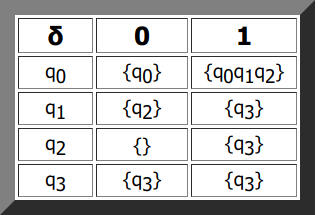
\includegraphics[width=0.45\textwidth]{Figure/table1.png}
    }
    \subfigure[表2\#2]
	{
		\label{fig:sub2}		
		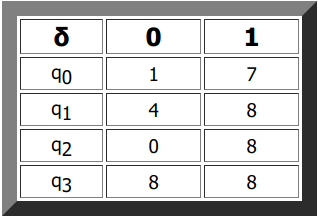
\includegraphics[width=0.45\textwidth]{Figure/table2.png}
	}
	\caption{转移函数δ表格描述}
	\label{fig:subfigure}
\end{figure}
你的任务,是要将一个给定的NFA转换为一个完全等价的DFA(有限状态自动机等价的意思是识别相同的语言)。这里我们约定自动机识别的字符集为{0,1},初始状态集合为Q0,状态集为{q0,q1,…,qn-1}。

\subsection{Input}
输入第一行只有一个正整数t,表示有t个测试数据(意味着t个NFA)t≤10;
对于每组测试数据(每个NFA),首先是3个正整数n,Q0,f,分别表示状态数、起始状态集合和接受状态集合的特征串对应的整数。n≤10;Q0,f < 2n;
接下来两行是NFA的转移函数矩阵,第一行是每个状态在输入为0的状态转移情况,用特征串对应的整数表示;第二行是每个状态在输入为1的状态转移情况。


\subsection{Output}
对于每个NFA,输出四行表示与之等价的DFA。输出格式如下:
第一行3个空格隔开的整数a b c,分别表示DFA的状态数,接受状态数,起始状态的编号(从0开始对状态编号)。要求 a < 65536。
b,c ≤ a 第二行b个空格分隔的整数,表示每个接收状态的编号,每个编号的值一定在[0,a)之间。
第三行、第四行每行a个空格分隔的整数,表示DFA的转移函数矩阵,第三行第i个值ui表示状态转移函数的一项δ(qi,0)→ui,第四行第i个值vi表示状态转移函数的一项δ(qi,1)→vi,,每个ui,vi的值一定在[0,a)之间。

\subsection{Sample Input}

\noindent1
\\4 1 8
\\1 4 0 8
\\7 8 8 8
\subsection{Sample Output}
\noindent16 8 1
\\8 9 10 11 12 13 14 15
\\0 1 4 5 0 1 4 5 8 9 12 13 8 9 12 13
\\0 7 8 15 8 15 8 15 8 15 8 15 8 15 8 15
\subsection{Judge Tips}
样例中的NFA如图一所示
与某个NFA等价的DFA不一定是唯一的,比如和图一等价的DFA可以是样例的解答,也可以是如下的DFA
\\4 1 0
\\3
\\0 2 0 3
\\1 3 3 3
\\本题会使用special judge,只要是符合条件的解答都可以接受(Accept)。
% 实验环境:Environment
\section{Lab Environment 环境}
\begin{itemize}
    \item 操作系统:Arch Linux
    \item 程序运行环境:gcc (GCC) 10.2.0
    % \item Python库(标准库未列出):numpy, pandas, matplotlib, sklearn
    \item 报告编写环境:TeX Live 2020
    \item 开发工具: VSCode
\end{itemize}
\newpage
% 实验步骤:Steps
\section{Lab Steps 步骤}
\subsection{分析问题}
对于NFA转DFA的问题,常用子集法求解,可以通过求闭包的方式求得DFA的状态,然后编号即可求解问题。
但是在本题中,起始状态集合和接受状态集合都是用特征串对应的整数所表示的,举个例子:状态集合的子集{q0q1q2},其特征串就是0111,而子集{q0},其特征串就是0001。将对应的特征串转换为十进制的数字
\\在本题中,我们直接使用子集法可能并不是最佳的解题方法,因为特征串用递归的方式处理往往会更加方便!

\subsection{算法思想}

\begin{enumerate}
    \item 状态集合的子集合,采用二进制(特征)串的方式,一个子集中包含该状态,对应的特征串就为1,否则为0,比如上面状态集合的子集{q0q1q2},其特征串就是0111,而子集{q0},其特征串就是0001。
    \item 采用DFS的方式搜索整个状态图。
    \item 搜索过程中,对于每一个特征串p,用p $\oplus$ $-$p取出p的最后一个状态(最低非零位),分别根据状态转换表格搜索0,1到达的集合,维护到达状态序列Qlist和下标。
    \item 标记已访问过的状态,直到整个状态图搜索结束,根据记录的序列和下标调整标号,打印结果。
\end{enumerate}
\subsubsection{对特征串的处理:}
\begin{itemize}
    \item x$\wedge $ $-$x: lowbit运算,返回最低位1表示的值
    \item lowbit x $\oplus$ x运算: 剔除最低位的1
\end{itemize}

\newpage
\subsubsection{算法伪代码表述:}
经过上述分析,算法伪代码可以表述为:
\lstinputlisting[language=c]
{./Code/mind.cpp}


\newpage
% 实验结果:Results
\section{Lab Results 结果}
\subsection{实验结果}

\begin{figure}[htbp]	% 浮动
    \centering
    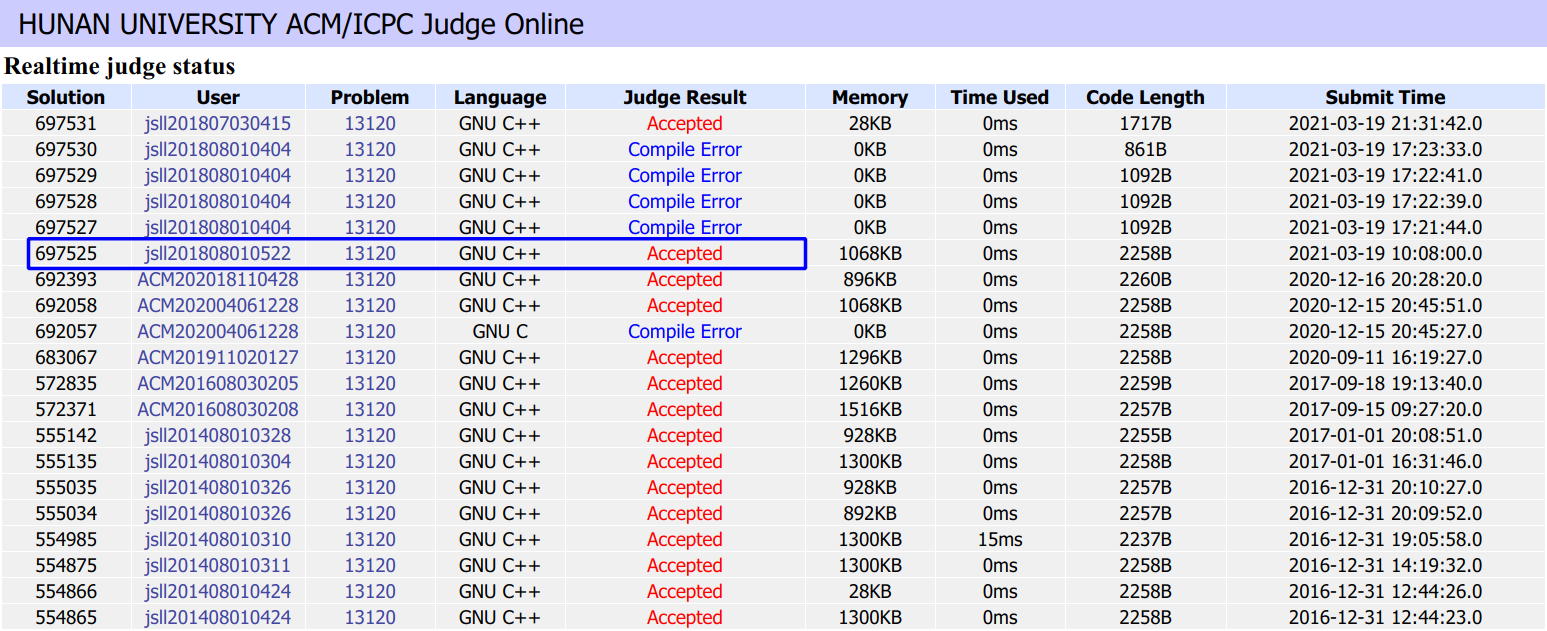
\includegraphics[width=1\linewidth]{Figure/solution.png}
    \caption{http://acm.hnu.cn/online 提交结果}
    \label{fig:figure1latexintro}
\end{figure}
在http://acm.hnu.cn/online提交代码,AC通过. SolutionID 697525,User jsll201808010522,	
Memory 3072KB	Time Used 0ms。因此,实验正确。
% 实验心得:Experience
\section{Lab Experience 心得}
\subsection{实验心得}
\begin{enumerate}
    \item 本次实验难度适中,因为在教材中都能找到NFA确定化和DFA最小的的算法。
    子集法虽然很容易理解,但是在算法实现过程中仍然有很多需要注意的地方。
    在本题中,由于起始状态集合和接受状态集合都是用特征串对应的整数所表示,子集法可能并不是最佳的解题方法,因为特征串用递归的方式处理往往会更加方便。
    \item 对特征串的处理也值得注意:
    \begin{itemize}
        \item x$\wedge $ $-$x: lowbit运算,返回最低位1表示的值
        \item lowbit x $\oplus$ x运算: 剔除最低位的1
    \end{itemize}
\end{enumerate}
\appendix
% 附录
\newpage
\section{附录1:Solution}
\begin{lstlisting}[language=c]
    #include<iostream>
    #include<cmath>
    #include<cstring>
    #define M 1000000
    using namespace std;
    int Qlist[M];                       //状态序列,记录的是NFA状态号     
    int transTable0[M],transTable1[M];  //读取0 / 1对应的转移矩阵
    int lft[M];                         //左子集合
    int rgt[M];                         //右子集合
    int QlistAdjust[M];                 //状态序列,记录的是DFA状态号
    bool visit[M];                      //标记为已经访问
    bool ac[M];                         //接受状态集合
    int cnt, n, q, f;
    // 将十进制p转化为二进制位对应的下标
    int indexOfBinary(int p){
        int x = 1;
        if(p == 1)
            return 0;
        int i = 0;
        while(++i)
        {
            x <<= 1;
            if(p == x) return i;
        }
        return 0;
    }
    // a:sum , b:状态号
    int travel(int a, int b){
        while(b){
            int x = b&(-b);                     // b的一个状态x = q
            if(!(a&x))                          // 如果a&x = 0,表示sum中不含x状态,用 ^ 添加
                a ^= x;             
            b ^= x;                             // 剔除b中的的x状态
        }
        return a;                               // 返回a的结果,表示b能到达的子集合
    }
    // 搜索状态图,从起始位置p开始
    void DFS(int p){
        Qlist[cnt] = p;
        int lsum = 0, rsum = 0;
        while(p){
            int x = p&(-p);                     // 选择p的一个状态,我们才用与上p的补运算可以取出最后一个为1的位
            int y = indexOfBinary(x);           // 状态x的下标位置
            lsum = travel(lsum, transTable0[y]);// 经过0到达的子集合
            rsum = travel(rsum, transTable1[y]);// 经过1到达的子集合
            p ^= x;                             // 迭代,p =p^x 剔除已经搜索的状态x,也就是最后一位
        }
        lft[cnt] = lsum;                        // 将DFA中的状态:δ(qcnt,0)保存
        rgt[cnt] = rsum;                        // 将DFA中的状态:δ(qcnt,1)保存
        cnt++;                                  // 指针移动到下一个DFA状态
        if(!visit[lsum])                        // 如果lsum还没有被访问,则要迭代访问lsum
            visit[lsum] = 1, DFS(lsum);
        if(!visit[rsum])                        // 同上
            visit[rsum] = 1, DFS(rsum);           
    }
    int main()
    {
        int t;                                  // t个测试数据
        scanf("%d", &t);                        
        while(t--)                              // 输入测试数据
        {
            scanf("%d%d%d", &n, &q, &f);        // 状态数,起始状态集合,接受状态集合的特征串对应的整数
            for(int i = 0; i < n; i++)          // 输入转移矩阵0 / 1
                scanf("%d", &transTable0[i]);
            for(int i = 0; i < n; i++)
                scanf("%d", &transTable1[i]);
            cnt = 0;
            memset(visit, 0, sizeof(visit));
            memset(ac, 0, sizeof(ac));
            visit[q] = 1;
            // 从起始状态开始搜索状态图
            DFS(q);
    
            // 遍历标记接收状态集合,sum表示当前接受状态个数
            int sum = 0;    
            for(int i = 0; i < cnt; i++)
                if(Qlist[i]&f) ac[i] = 1, sum++;    // 标记接受状态
            for(int i = 0; i < cnt; i++)
                QlistAdjust[Qlist[i]] = i;          // 将ans记录的NFA号调整到DFA上来 
            printf("%d %d %d\n", cnt, sum, 0);      // DFA的状态数,接受状态数,起始状态的编号
            for(int i = 0, j = 0; i < cnt; i++){    // 接收状态的编号
                if(ac[i]){
                    if(j)   printf(" ");
                    printf("%d", i);
                    j++;
                }
            }
            printf("\n");
            for(int i = 0; i < cnt; i++) {          // δ(qi,0)→ui
                if(i)   printf(" ");
                printf("%d", QlistAdjust[lft[i]]);
            }
            printf("\n");
            for(int i = 0; i < cnt; i++){           // δ(qi,1)→vi
                if(i) printf(" ");
                printf("%d", QlistAdjust[rgt[i]]);
            }
            printf("\n");
        }
        return 0;
    }
\end{lstlisting}

\end{document}
